\documentclass[12pt]{article}
\usepackage{graphicx} % Required for inserting images
\usepackage{setspace}
\usepackage[brazil]{babel}
\usepackage{amsmath}
\usepackage{amssymb}
\usepackage{amsfonts}
\usepackage{amsthm}
\usepackage{bm}
\usepackage[T1]{fontenc}
\usepackage[utf8]{inputenc}
\usepackage{xcolor}
\usepackage{tabularx}
\usepackage{fancyhdr}
\usepackage{float}
\usepackage[colorlinks=true, allcolors=blue]{hyperref}
\usepackage[bottom]{footmisc}
\usepackage{hyperref}
\usepackage{wrapfig}
\usepackage[shortlabels]{enumitem}
\usepackage[a4paper, margin=2.5cm]{geometry}
\usepackage{dsfont}
\usepackage{caption}
\usepackage{subcaption}

\newtheorem{prop}{Proposição}
\newtheorem{defi}{Definição}
\newtheorem{teo}{Teorema}
\newtheorem{coro}{Corolário}

\begin{document}
    
    \begin{titlepage} 
        \begin{titlepage}

    \begin{figure}
        \centering
        
\includegraphics[scale = 0.5]{FGV_logo}\label{fig:figure}
    \end{figure}

    {\fontfamily{lmr}\selectfont
    
    \begin{center}
        % Instituição 
        \vspace*{0.5cm}
        \scshape {\Large ESCOLA DE MATEMÁTICA APLICADA}

        % Disciplina
        \vspace*{3cm}
        {\Large Álgebra Linear}

        \vspace*{0.5cm}
        {\Large Docente: Yuri Fahham Saporito}

        % Título
        \vspace*{2cm}
        \doublespacing
        \textbf {\LARGE Eigenfaces: \\ Uma Análise Comparativa entre PCA e SVD}

        % Autores
        \vspace*{3cm}
        {\Large Beatriz Miranda Bezerra \\Gustavo Murilo Cavalcante Carvalho}


        \vspace*{5cm}
        {\large novembro de 2023}
    \end{center}
    }

\end{titlepage}
    \end{titlepage}
    \newpage
    
    \tableofcontents %sumário
    \newpage 
    
    \section{Introdução}
        
        
        A análise de componentes principais (PCA) e a decomposição de valores singulares (SVD)
        têm sido  extensivamente  aplicados  a  variadas áreas  da  computação: Mineração de Dados, Aprendizado de Máquina, Recuperação de Informação, Processamento Digital de Sinais, dentre outras. 
        
        
        Além disso, são técnicas amplamente empregadas na análise de eigenfaces, uma representação de faces humanas como combinações lineares de componentes principais. Embora ambas as abordagens compartilhem semelhanças conceituais, apresentam diferenças cruciais em sua aplicação. Este trabalho tem como objetivo explorar essas diferenças, destacando como o PCA e o SVD influenciam a representação de eigenfaces, fornecendo uma compreensão mais profunda das implicações práticas e teóricas dessas técnicas no reconhecimento facial.

    \section{Comparação entre SVD e PCA}
        \subsection{SVD} 
                \begin{itemize}
                    \item É o processo de fatoração de matrizes capaz de representar uma matriz de dados $A$ por meio de três outras matrizes $U$, $S$ e $V^{T}$ que representam, respectivamente:  uma  base  ortonormal para as colunas  de $A$ (autovetores  a esquerda), o conjunto de escalares que determinam a relevância de cada autovetor (autovalores); e uma base ortonormal para as linhas de $A$ (autovetores a direita). 
                    \item  Tem  por  objetivo  realizar  a  redução  de  posto  e  a  aproximacão  de  baixo-posto  de  uma  matriz $N$-dimensional. 
                    \item Objetivos: eficiência  de  manipulação  de dados matriciais; redução da dimensionalidade dos dados e remoção de ruídos dos dados originais.
                    \item Foca na descoberta de “identidades” predominantes dos dados (identidade de uma variável é sua média amostral).
                \end{itemize}
            \subsection{PCA} 
                \begin{itemize}
                    \item É uma técnica estatística multivariada que possui como objetivo explorar a estrutura de variabilidade dos dados. Preocupa-se  em  explicar  a  estrutura  de  variância-covariância de um conjunto de variáveis por meio de poucas combinações lineares entre essas variáveis. 
                    \item Os principais conceitos estatísticos para entender o processo são:
                        \begin{itemize}
                            \item Média: pode ser definida como uma medida que busca sintetizar a informação de tendência central da distribuição de valores da variável;
                            \item Variância: medida de dispersão estatística que indica o quão longe os valores de uma variável se encontram da média;
                            \item Covariância: serve para medir o grau de relacionamento linear entre duas variáveis.
                        \end{itemize}
                    \item Objetivos: redução de dados e interpretação.
                    \item Foca na descoberta de “distorções” marcantes nos dados (distorção de uma variável é sua variância amostral a partir de sua identidade). 
                    \item Resumidamente, as etapas para aplicação do PCA são:
                        \begin{enumerate}
                            \item Escolher variáveis (dimensões) a serem avaliadas;
                            \item Subtrair média de cada dimensão, produzindo um conjunto de dados com média zero;
                            \item Calcular matriz de covariância;
                            \item Calcular os autovetores e autovalores da matriz de covariância;
                            \item Escolher as $k$ componentes principais ($k$ autovetores com maior autovalor)
                            \item Interpretar as informaçõess contidas nas componentes principais.
                        \end{enumerate}
                        No entanto, é possível substituir a etapa $4$ pela aplicação do SVD, uma vez que os $k$ primeiros autovetores da matriz de covariância são as $k$ dimensões de maior variabilidade. Neste sentido, podemos interpretar o PCA como o processo de fatoração do SVD, aplicado à matriz de covariância.
                \end{itemize}
                 Assim, salvo as devidas diferenças teóricas, a questão prática se reduz à identificarmos as diferenças entre SVD sobre a matriz de covariância e SVD sobre a matriz original.
                   
    \section{Eigenfaces e aplicação em dados reais}
        Eigenface é um termo introduzido pela primeira vez por Sirovich e Kirby em 1987, que consiste em um conjunto de bases de características obtidas por meio da Análise de Componentes Principais (PCA), utilizando a Decomposição de Valores Singulares (SVD). Esse conjunto de bases é usado para projetar o espaço de imagens faciais de alta dimensão para uma dimensão inferior. Isso permite a criação de um conjunto de $r$ características básicas, chamadas de "eigenpictures" ou, neste caso, "eigenfaces", que podem ser usadas em combinações lineares para representar o número total de $n$ imagens faciais, onde $r$ é menor que $n$.
    
        O Eigenface é um conceito fundamental utilizado no reconhecimento facial. Posteriormente, diversos algoritmos de pré-processamento, como a correção gamma para o pré-processamento de iluminação, foram desenvolvidos com base nele para melhorar a precisão do reconhecimento facial. Basicamente, quando uma nova imagem é introduzida no sistema, ela é projetada no subespaço gerado por essas eigenfaces e, a partir dessa projeção, é classificada com base na sua posição relativa em relação às projeções de indivíduos já conhecidos. Esse processo permite identificar a pessoa correspondente à imagem com base nas características faciais extraídas de forma automatizada.

         \begin{figure}[H]
              \centering
              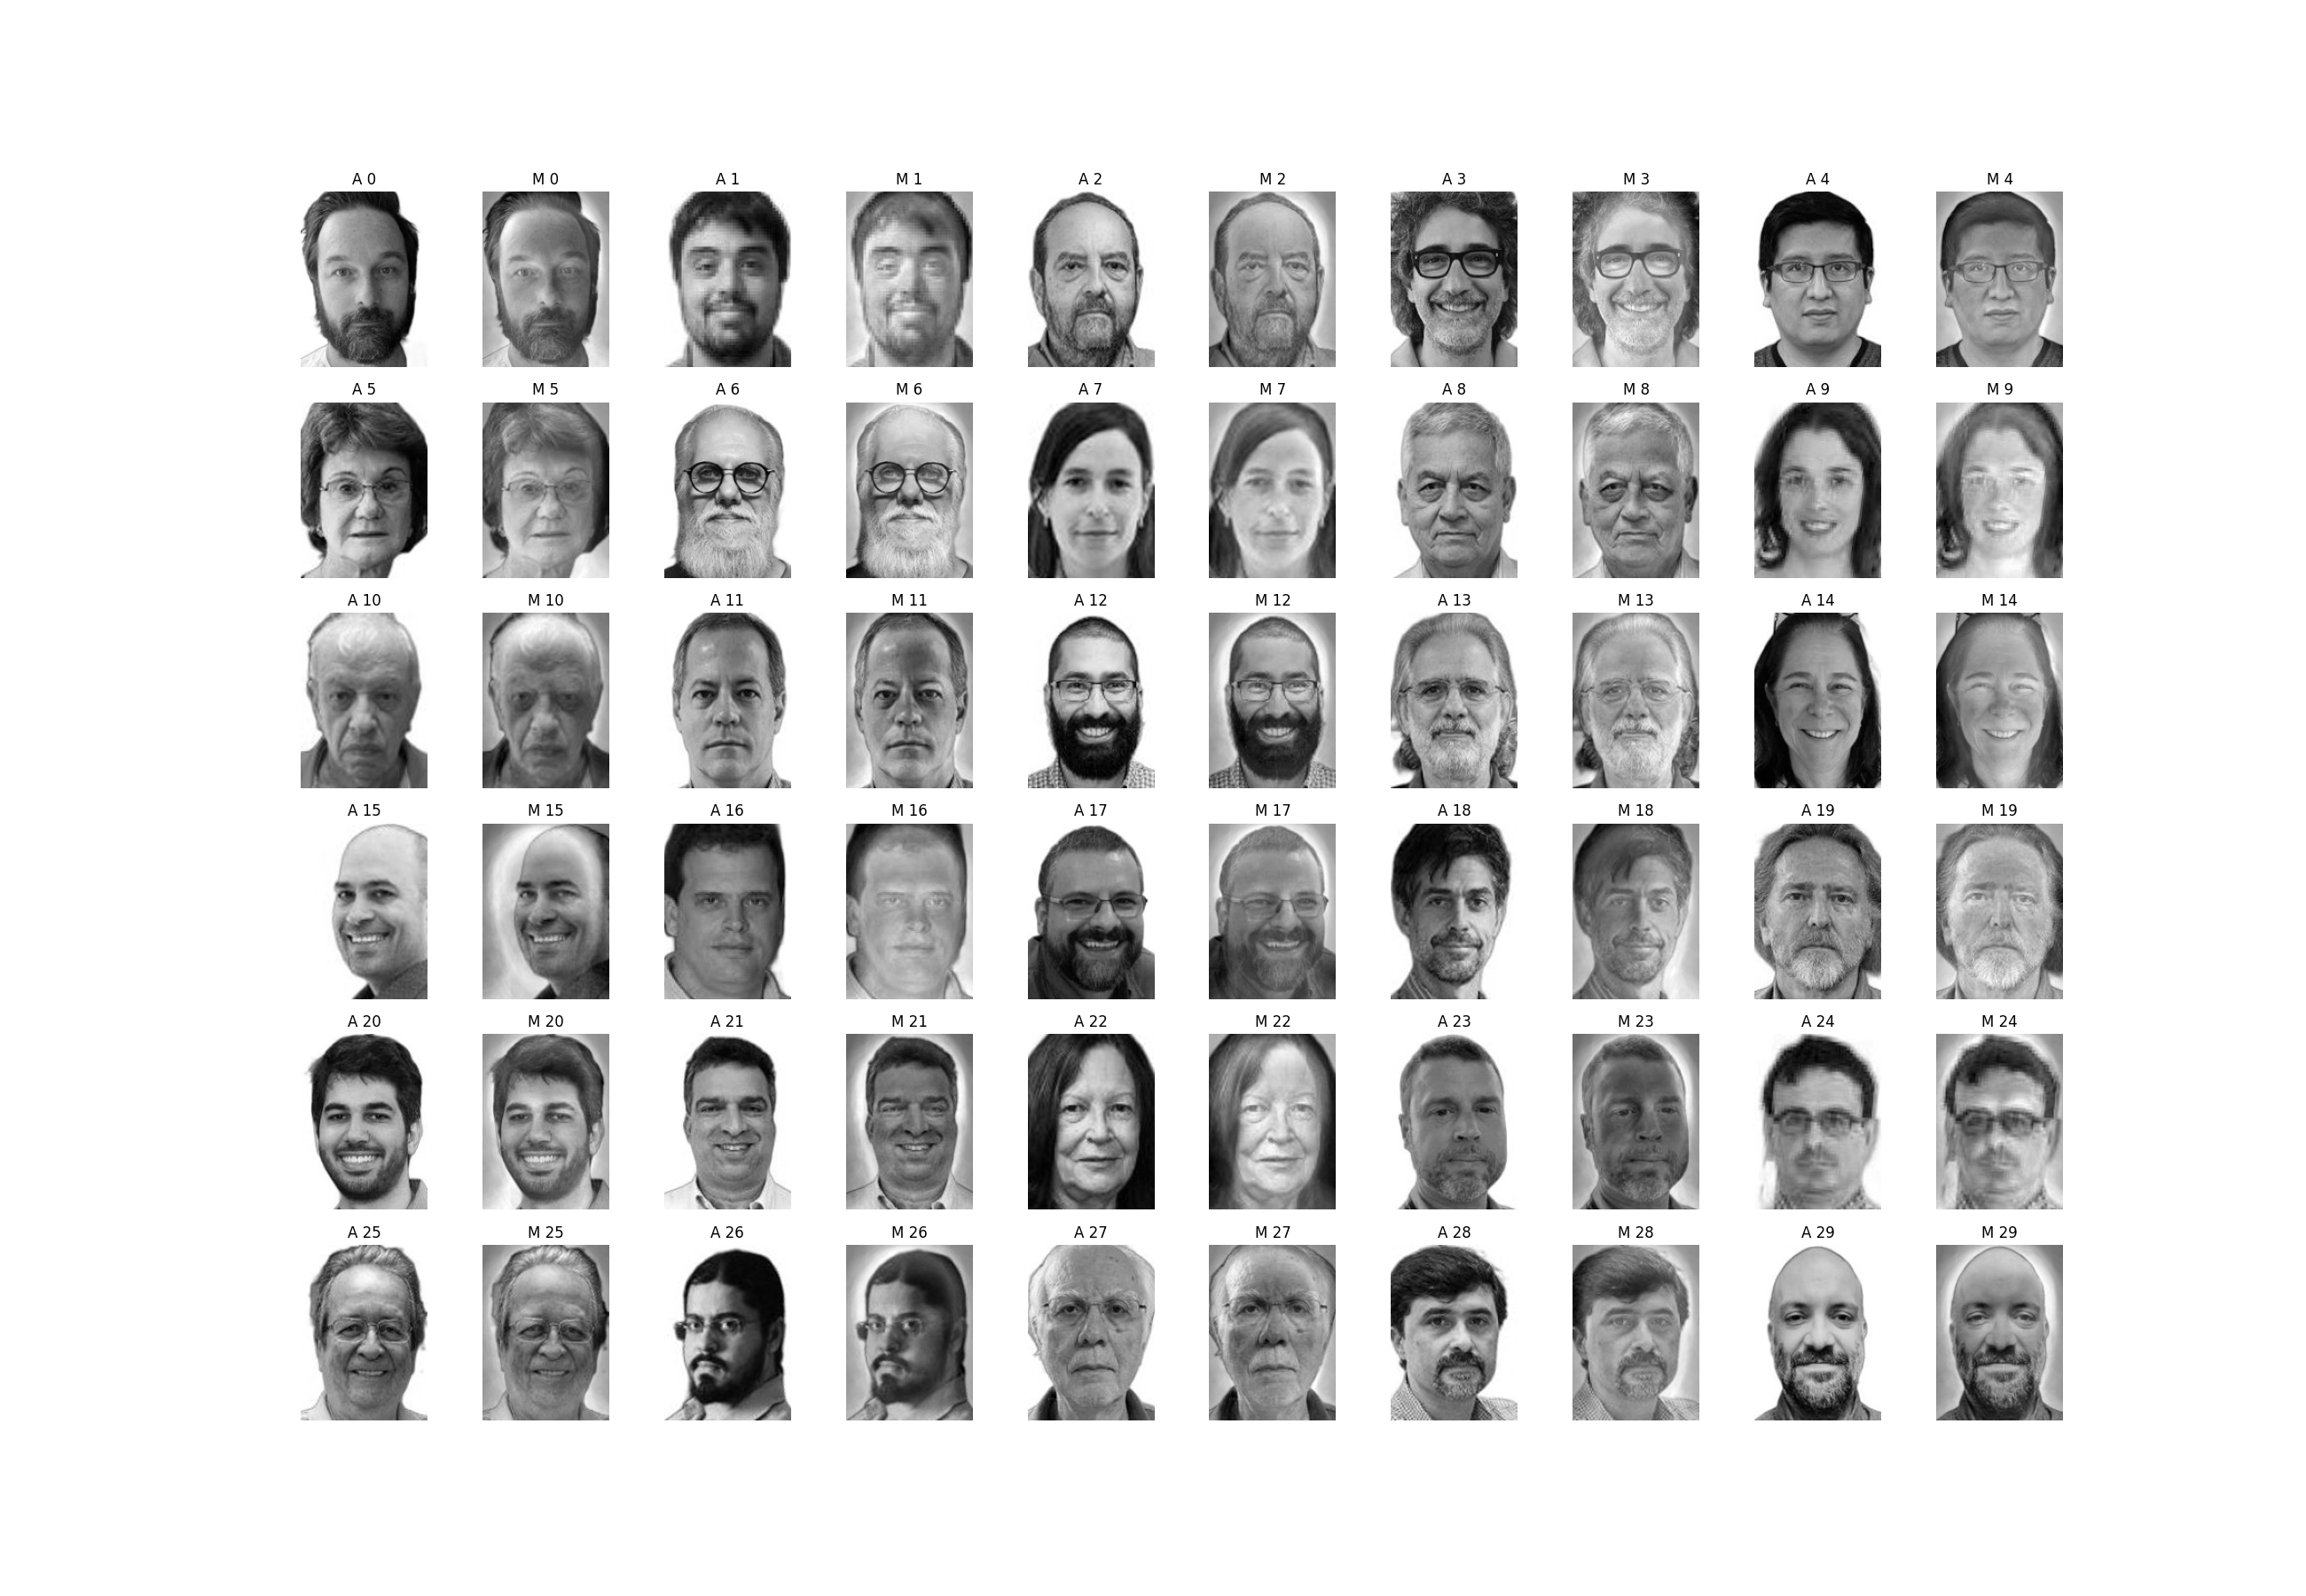
\includegraphics[width=1\textwidth]{img/EMAP_1.png}
              \caption{Exemplo de imagens com suas respectivas correções pela média.}
              \label{fig:exemplo}
        \end{figure}
        

        Uma imagem em preto e branco com resolução $m \times n$ pode ser representada de forma matricial, de modo que seus elementos sejam valores na escala de cinza. Para trabalhar melhor com o conjunto de imagens, as linhas da imagem são enfileiradas formando um vetor $1 \times mn$, que é então transposto. 


        Definimos então a $i$-ésima imagem como $\boldsymbol{a_i} \in \mathds{R}^{mn}$ tal que $1 \leq i \leq q$, onde $q$ é o número de imagens no banco de dados. A partir delas, é criada a matriz que contém todas as imagens originais, $\boldsymbol{A} \in \mathds{R}^{mn \times q}$.
        
            $$
            \boldsymbol{A} = \begin{bmatrix} \boldsymbol{a_1} & \boldsymbol{a_1} & \ldots & \boldsymbol{a_q} \end{bmatrix}
            $$

        Como queremos analisar a variabilidade dos dados, inicialmente devemos centralizá-los, eliminando características que são comuns a todas as imagens. 
        
        Essa identidade é encontrada na face média $\boldsymbol{f_\mu}$, a média aritmética de todas as imagens no conjunto de dados.
        
            $$
            \boldsymbol{f_\mu} = \frac{1}{q} \sum_{i=1}^{q} \boldsymbol{a_i}
            $$

        \begin{figure}[H]
              \begin{subfigure}{0.35\textwidth}
                \centering
                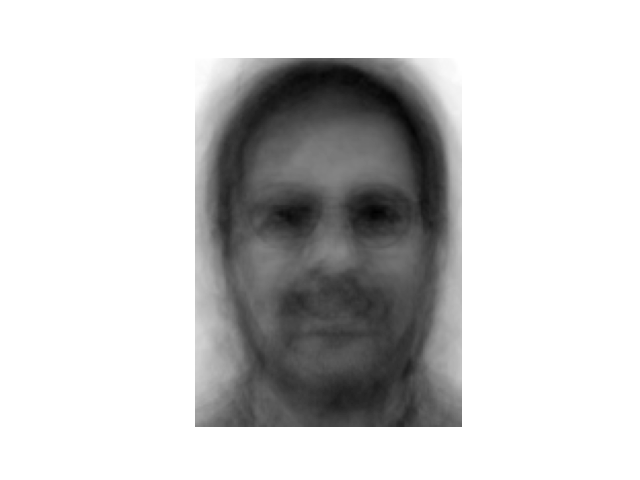
\includegraphics[width=\textwidth]{img/EMAP_0.png}
                \caption{Corpo docente da EMAp.}
                \label{fig:imagem1}
              \end{subfigure}
              \hfill
              \begin{subfigure}{0.35\textwidth}
                \centering
                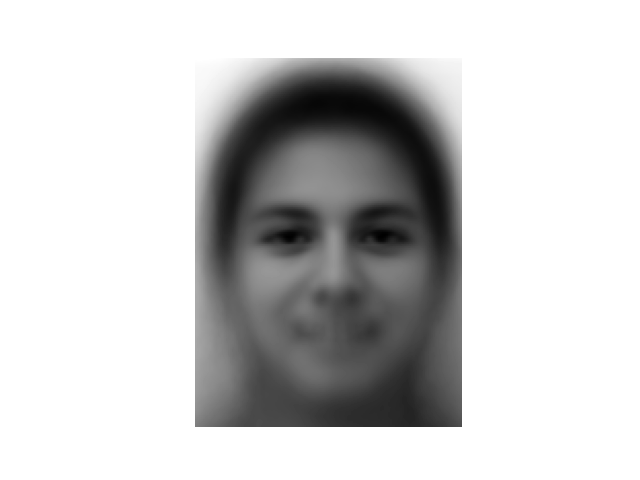
\includegraphics[width=\textwidth]{img/MAIN_0.png}
                \caption{FEI Face Database.}
                \label{fig:imagem2}
              \end{subfigure}
              \caption{Face média}
            \end{figure}
            
        Em seguida, definimos a matriz com os dados centralizados $\boldsymbol{M}$ por:

            $$
            \boldsymbol{m_i} = \sum_{i=1}^{q} \boldsymbol{a_i} - \boldsymbol{f_\mu}
            $$        

            $$
            \boldsymbol{M} = \begin{bmatrix} \boldsymbol{m_1} & \boldsymbol{m_2} & \ldots & \boldsymbol{m_q} \end{bmatrix}
            $$

            
           A matriz de covariância amostral do nosso conjunto de dados, denotada por $\boldsymbol{C} \in  \mathds{R}^{mn \times mn}$ pode ser calculada da seguinte maneira:

            $$
            \boldsymbol{C} 
            = \frac{1}{q-1} \sum_{i=1}^{q}  (\boldsymbol{a_i} - \boldsymbol{f_\mu}) (\boldsymbol{a_i} - \boldsymbol{f_\mu} )^{T}
            = \frac{1}{q-1} \boldsymbol{M} \boldsymbol{M}^T 
            $$
            
            Nesta fórmula, $\boldsymbol{C}$ representa a matriz de covariância. M é a matriz dos dados, $q$ é o número de observações no conjunto de dados, $\boldsymbol{a_i}$ são os vetores de observação, $\boldsymbol{f_\mu}$ é o vetor de médias das observações, e $(\boldsymbol{a_i} - \boldsymbol{f_\mu}) (\boldsymbol{a_i} - \boldsymbol{f_\mu})^T$ representa o produto externo dos desvios das observações em relação à média. A matriz de covariância é uma medida importante da relação entre as diferentes variáveis no conjunto de dados.

            \begin{figure}[H]
                  \centering
                  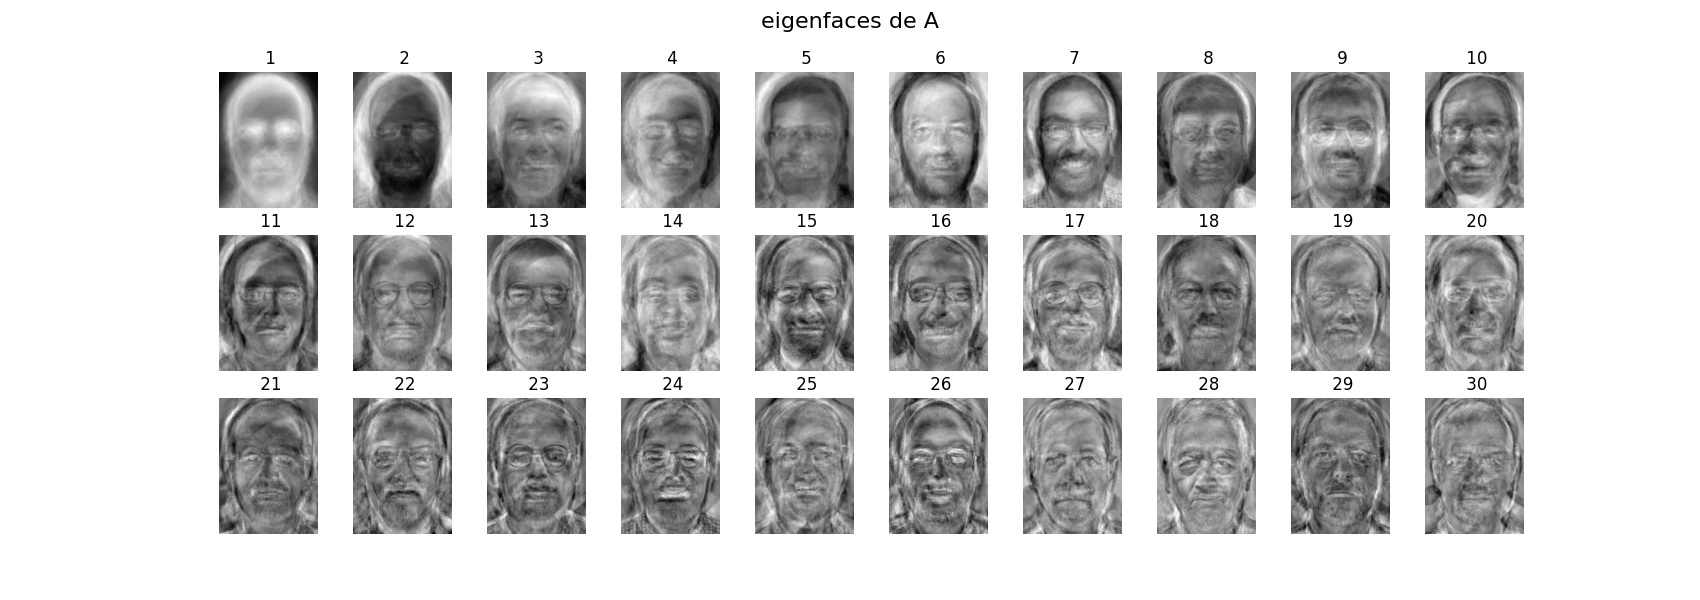
\includegraphics[width=1\textwidth]{img/EMAP_2.png}
                  \caption{Eigenfaces de A}
                  \label{fig:exemplo}
            \end{figure}
            
            \begin{figure}[H]
                  \centering
                  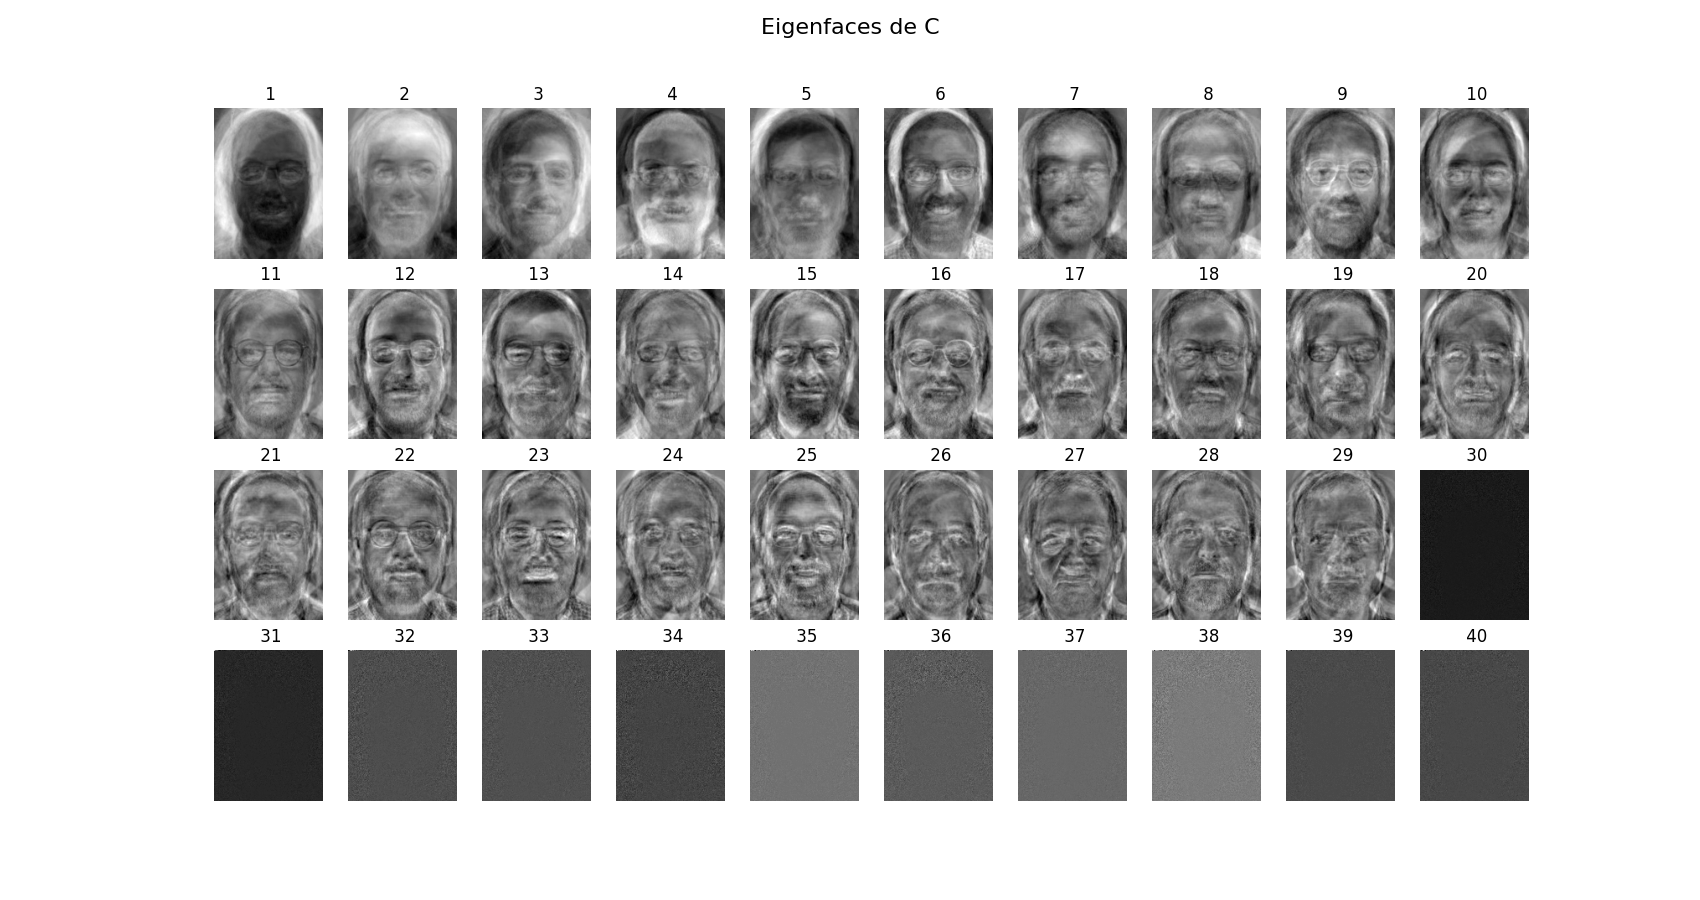
\includegraphics[width=1\textwidth]{img/EMAP_3.png}
                  \caption{Eigenfaces de C}
                  \label{fig:exemplo}
            \end{figure}

            Vale ressaltar que $\boldsymbol{C}$ é simétrica e positiva definida, portanto, aplica-se o teorema espectral. A próxima etapa envolve a decomposição da matriz de covariância $\boldsymbol{C}$ usando a SVD, que é dada por:

            $$
            \boldsymbol{C} = \boldsymbol{U} \boldsymbol{\Sigma} \boldsymbol{V}^{T}  = \boldsymbol{U} \boldsymbol{\Sigma} \boldsymbol{U}^{T}
            $$

            onde $\boldsymbol{U}$ é a matriz de autovetores e $\boldsymbol{\Sigma}$ é uma matriz diagonal contendo os autovalores em ordem decrescente. Os autovetores em $\boldsymbol{U}$ são chamados de "eigenfaces". Eles representam as principais componentes de variação nas imagens faciais.

            Repare bem nas Eigenfaces mais relevantes geradas por cada matriz:

            \begin{figure}[H]
                  \centering
                  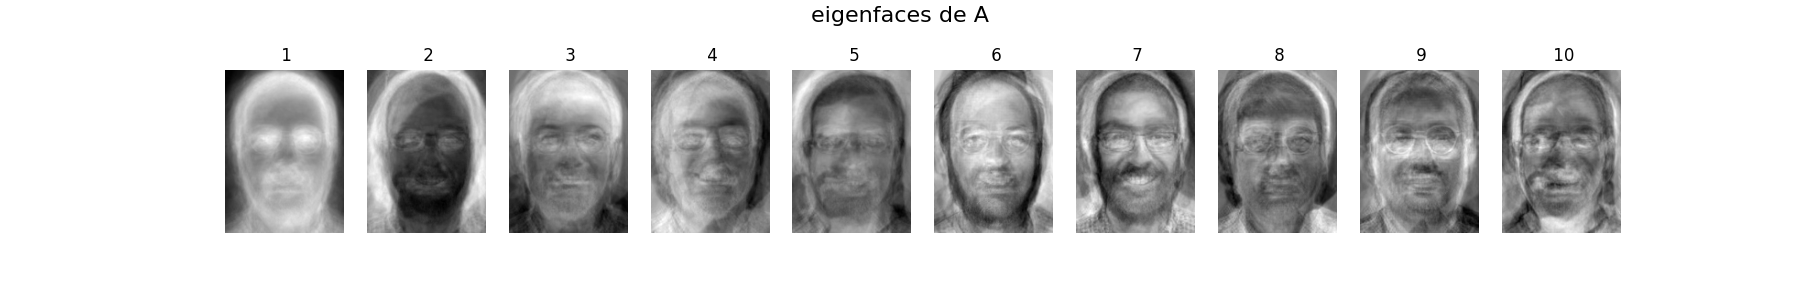
\includegraphics[width=1\textwidth]{img/EMAP_4.png}
                  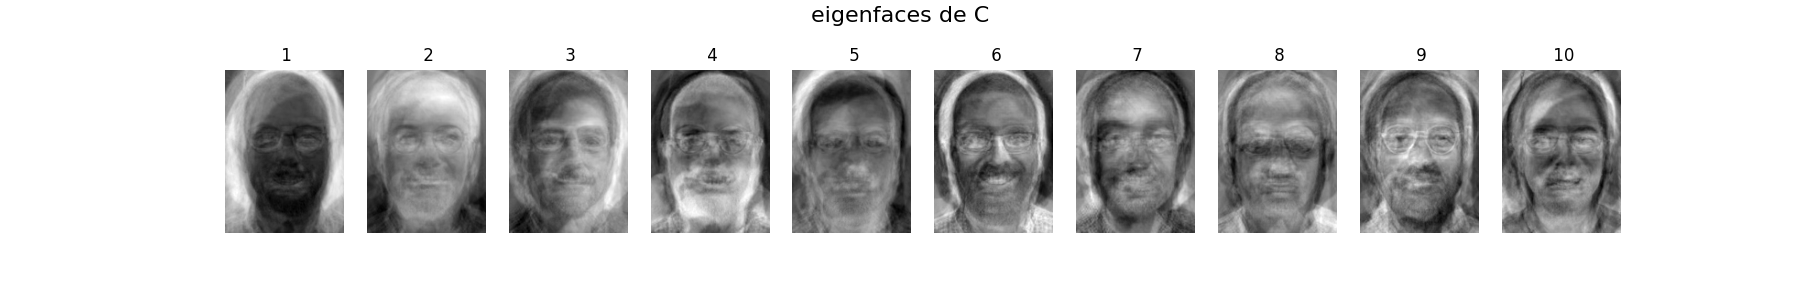
\includegraphics[width=1\textwidth]{img/EMAP_5.png}
                  \caption{Eigenfaces mais relevantes de cada matriz}
                  \label{fig:exemplo}
            \end{figure}

            

            Para reconhecer um rosto novo, é necessário projetar a imagem desse rosto nas eigenfaces para obter os coeficientes de projeção. Seja $\boldsymbol{z}$ o vetor de coeficientes de projeção de uma imagem de teste. Podemos calcular $\boldsymbol{z}$ da seguinte maneira:
 
            $$
            \boldsymbol{z} = \boldsymbol{U}^{T}(\boldsymbol{x_{teste}} - \boldsymbol{F_\mu})
            $$


            onde $\boldsymbol{x_{teste}}$ é o vetor de pixels da imagem de teste.

            Finalmente, podemos comparar $\boldsymbol{z}$ com os coeficientes de projeção das imagens de treinamento para identificar a imagem mais próxima ou realizar uma classificação com base em alguma métrica de distância, como a distância euclidiana. Entretanto, na prática, existem várias otimizações e variações dessa técnica para melhorar o desempenho e a precisão do reconhecimento facial.
            
        
    \section{Discussão dos resultados e conclusão}
        Suponha que queremos reconstruir a seguinte imagem:

        \begin{figure}[H]
                  \centering
                  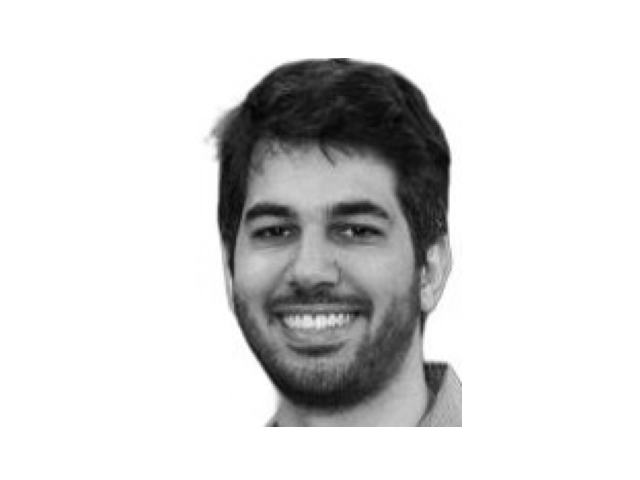
\includegraphics[width=0.5\textwidth]{img/MAIN_6.png}
                  \caption{Imagem a ser reconstruída}
                  \label{fig:exemplo}
        \end{figure}
        
        \begin{figure}[H]
                  \centering
                  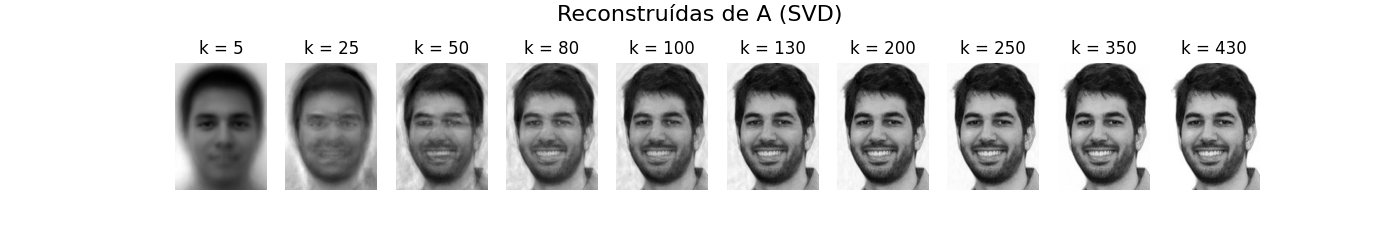
\includegraphics[width=1\textwidth]{img/MAIN_7.png}
                  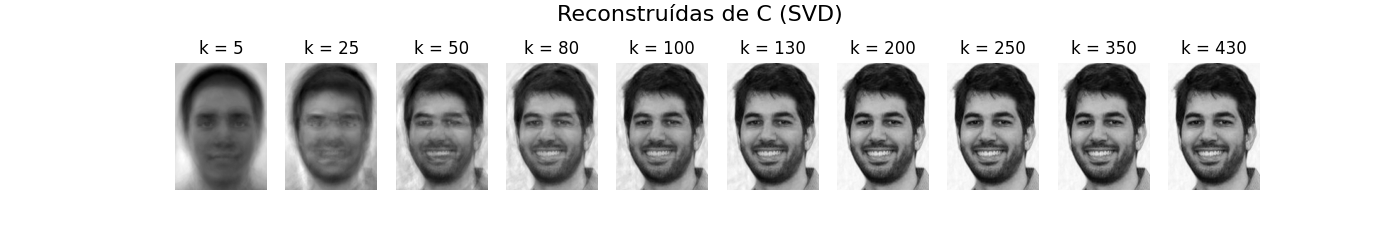
\includegraphics[width=1\textwidth]{img/MAIN_8.png}
                  \caption{Imagem reconstruída}
                  \label{fig:exemplo}
        \end{figure}

        \begin{figure}[H]
              \begin{subfigure}{0.5\textwidth}
                \centering
                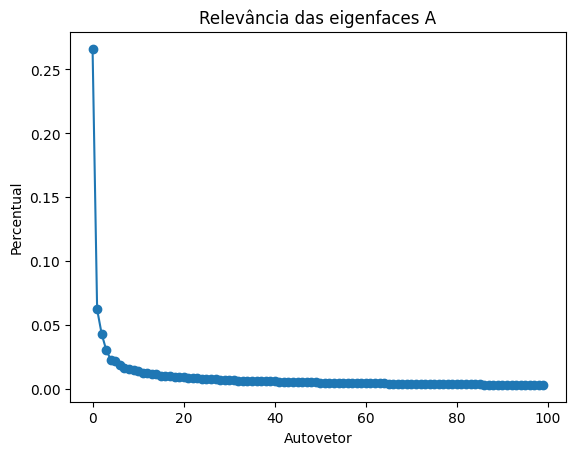
\includegraphics[width=\textwidth]{img/MAIN_10.png}
                \label{fig:imagem1}
              \end{subfigure}
              \hfill
              \begin{subfigure}{0.5\textwidth}
                \centering
                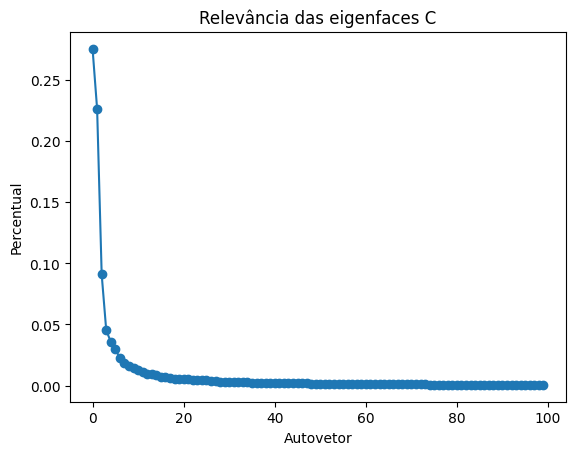
\includegraphics[width=\textwidth]{img/MAIN_11.png}
                \label{fig:imagem2}
              \end{subfigure}
              \caption{Relevância das Eigenfaces de cada matriz}
        \end{figure}

        \begin{figure}[H]
                  \centering
                  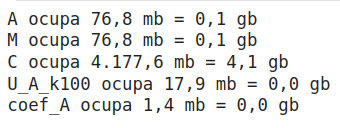
\includegraphics[width=0.5\textwidth]{img/memoria_ocupada.png}
                  \caption{Memória ocupada por cada matriz}
                  \label{fig:exemplo}
        \end{figure}

        Como visto acima, o resultado dos dois processos é idêntico. A diferença entre eles é que é muito menos custoso computacionalmente manter e fazer a decomposição SVD da matriz A do que fazer o mesmo com a matriz de covariância C. Assim, embora a grande maioria dos estudos  adotem  o  PCA  para  a  tarefa  de  reconhecimento  facial,  o  SVD,  parece muito mais apropriado.

    
    
    % adiciona Referências
    \newpage
    \nocite{*}
    \bibliography{sample.bib}{}
    \bibliographystyle{plain}  

\end{document}
